\documentclass[a4paper,12pt]{extreport}
\usepackage[utf8]{inputenc}
\usepackage[russian]{babel}
\usepackage{ragged2e}
\usepackage[mag=1000,a4paper,left=1cm,right=1cm,top=1cm,bottom=1cm,noheadfoot]{geometry}
\usepackage{mathtext}
\usepackage{amsmath,amssymb,amsthm,amscd,amsfonts,graphicx,epsfig,textcomp,wrapfig}
\usepackage[dvips]{graphicx}
\graphicspath{{noiseimages/}}

\newcommand{\tab}{\hspace{10mm}}
\newcommand{\name}{
			\normalsize
			{
				\ \ \quad
                \mbox{} \hfil {\flushleft{Взлет}} \hfill {04.11.2023}
			%\quad
			}
			\vspace{5pt}\hrule
		}

\def\head#1#2{
	\begin{center}{
			\LARGE
			\bf #2
			
			{\normalsize \bf #1}
			\vspace{-10pt}
	}\end{center}
}

\newcommand{\del}{\mathop{\raisebox{-2pt}{\vdots}}}
\newcommand{\q}{}

\newcounter{tasknum}
\setcounter{tasknum}{0}
\def\thetasknum{{\textbf{\arabic{tasknum}}}}
\newcommand{\task}{\refstepcounter{tasknum}\vspace{2pt}\noindent \textbf{} \thetasknum\textbf{.}~}
\newcommand{\coff}{\refstepcounter{tasknum}\vspace{2pt}\noindent \textbf{Задача} \thetasknum *\textbf{.}~}


\newcommand{\eq}[1]{\underset{#1}{\equiv}}
\newcommand{\dv}{\ensuremath{\mathop{\raisebox{-2pt}{\vdots}}}}
\newcommand{\ndv}{\not \dv}

\newcounter{exnum}
\setcounter{exnum}{0}
\def\theexnum{{\emph{\arabic{exnum}}}}
\newcommand{\ex}{\refstepcounter{exnum}\vspace{2pt}\noindent \emph{Упражнение} \theexnum\emph{.}~}



\theoremstyle{plain}
\newtheorem{theorem}{Теорема}
\newtheorem{lemma}{Лемма}
\newtheorem{proposition}{Предложение}
\newtheorem{corollary}{Следствие}
\theoremstyle{definition}
\newtheorem{definition}{Определение}
\theoremstyle{remark}
\newtheorem{remark}{Замечание}
\newtheorem{example}{Пример}

\textheight=300mm %
\textwidth=180mm %
\oddsidemargin=-10.4mm%
\evensidemargin=-10.4mm %
\topmargin=-24.4mm


\begin{document}
	\pagestyle{empty}
    \name{}
	\head{8 класс}{КГ}
	\bigskip

\task Плоскость раскрашена в два цвета. Докажите, что найдутся две точки одного цвета на расстоянии $2023$ м.\\
	
\task Приведите пример выпуклого шестиугольника с $6$ диаметрами, ни один из которых не является стороной.\\

\task На плоскости отмечено $n$ точек. Докажите, что можно провести несамопересекающуюся ломаную, проходящую через все эти точки.\\

\task Множество отрезков на прямой таковы, что любые два из них имеют общую точку. Докажите, что они все пересекаются в одной точке.\\

\task На плоскости нарисовано несколько многоугольников, каждые два из которых имеют общую точку. Докажите, что найдётся прямая, пересекающая все эти многоугольники.\\

\task Какое наибольшее число диаметров может быть у плоского $N$-угольника?\\

\task Докажите, что для любого выпуклого многоугольника есть два гомотетичных с коэффициентом $2$ параллелограмма, один из которых содержит многоугольник, а другой содержится в нем.\\

\task Докажите, что для множества из $14$ точек общего положения есть как минимум $400$ способов разбить их на пары так, что если соединить точки в парах отрезками, то эти отрезки окажутся попарно непересекающимися.\\

\task Существуют ли три равных девятиугольника, все вершины которых совпадают, а все стороны – нет?\\

\task На плоскости дано $n$ точек общего положения. Проводится прямая через одну из точек и начинает вращаться вокруг нее по часовой стрелке, пока не встретит следующую точку. Затем она начинает вращаться вокруг нее и т. д. Докажите, что можно провести изначально прямую так, что она пройдет через все точки бесконечное число раз.\\

\task Докажите, что из любого конечного множества точек на плоскости можно так удалить одну точку, что оставшееся множество можно разбить на два множества, диаметры которых меньше диаметра первоначального множества.\\

\task На плоскости отмечено $2n$ точек общего положения. Докажите, что их можно разбить на два множества с одинаковым числом вершин в выпуклой оболочке.

\begin{figure}[h]
    \centering
    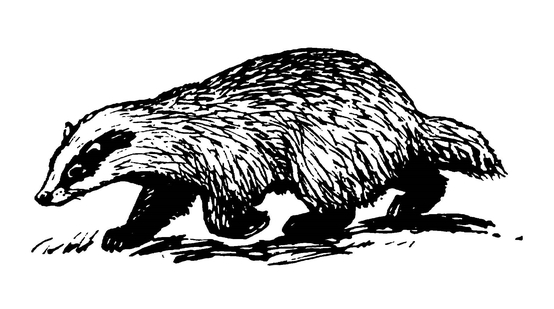
\includegraphics[width=0.45\linewidth]{барсук.jpeg}
\end{figure}

\end{document}
